% Created 2026-04-16 Thu 22:50
% Intended LaTeX compiler: pdflatex
\documentclass[11pt]{article}
\usepackage[utf8]{inputenc}
\usepackage[T1]{fontenc}
\usepackage{graphicx}
\usepackage{longtable}
\usepackage{wrapfig}
\usepackage{rotating}
\usepackage[normalem]{ulem}
\usepackage{amsmath}
\usepackage{amssymb}
\usepackage{capt-of}
\usepackage{hyperref}
\author{Sebastián Josué Zúñiga Mendoza}
\date{\today}
\title{}
\hypersetup{
 pdfauthor={Sebastián Josué Zúñiga Mendoza},
 pdftitle={},
 pdfkeywords={},
 pdfsubject={},
 pdfcreator={Emacs 29.3 (Org mode 9.6.15)}, 
 pdflang={English}}
\begin{document}

\tableofcontents

\section*{Sistemas Numéricos}
\subsection{Que es un número?}
Un número se refiere a una cadena de dígitos en donde la posición de
cada uno determina la base con la que se esté trabajando. Por ejemplo,
en el número 314.56:
\begin{itemize}
\item El 3 ocupa la base 2
\item El 1 ocupa la base 1
\item El 4 ocupa la base 0
\item El 5 ocupa la base -1
\item El 6 ocupa la base -2
\end{itemize}
De esta forma, la posición del número posee un peso r\textsuperscript{i}, donde r es
la base del sistema de numeración.

Por lo tanto, un número N en base r se expresa como:

\begin{figure}[htbp]
\centering
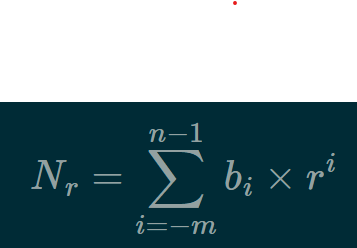
\includegraphics[scale=0.75]{./imagenes/sistemas_numeracion.png}
\caption{\label{fig:org45cbb24}SistemasNumeracion}
\end{figure}      

\textbf{Número en base 7: 345}

\textbf{Número en base 4: 12}

El valor correspondiente al número 345 en base 7 es 180. Por otro
lado, el valor correspondiente al número 12 en base 4 es 6.

Recordar que, en el caso del sistema de numeración decimal, la base
$$r = 10$$
\end{document}
